\chapter{Reti Bayesiane} \label{cap:RetiBayesiane}
\section{Introduzione}
Le reti bayesiane sono un \textbf{modello grafico probabilistico} che rappresenta
le relazioni probabilistiche tra un insieme di variabili. Queste reti sono utili
per rappresentare le relazioni di dipendenza tra le variabili e per effettuare
inferenze su di esse. Le dipendenze espresse graficamente dalle reti Bayesiane sono
solo assunzioni sul dominio, dal momento che vengono stimate usando algoritmi o
usando l'esperienza delle persone afferenti al dominio.

Usando l'indipendenza e l'indipendenza condizionata il modello causale è molto
più compatto, il numero di parametri utilizzato si riduce.
\begin{definizione}[\textbf{Rete Bayesiana}]
    Una \textbf{rete bayesiana} è un \textbf{grafo orientato aciclico} in cui i nodi sono
    annotati con una \textbf{informazione quantitativa}, ovvero la tabella di probabilità
    condizionata, e gli archi definiscono la \textbf{dipendenza e indipendenza condizionale}
    tra le variabili rappresentate dai nodi.
\end{definizione}
\begin{nota}
    Le variabili rappresentate dai nodi possono essere continue o discrete.
\end{nota}

Di norma diremo che se esiste l'arco $(x,y)\in E$ allora $x$ causa $y$ quindi
$x$ è genitore di $y$ e che $y$ è figlio di $x$.
\begin{center}
    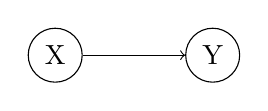
\begin{tikzpicture}
        \node[shape=circle,draw=black] (X) at (0,0) {X};
        \node[shape=circle,draw=black] (Y) at (2,0) {Y};
        \path [->] (X) edge node {} (Y);
    \end{tikzpicture}
\end{center}

La topologia della rete, ovvero la sua struttura, e le probabilità condizionate
dei nodi dati i loro genitori sono sufficienti a specificare la distribuzione
congiunta di tutte le variabili rappresentate dalla rete.

La componente quantitativa contenuta in ogni nodo è costituita da un insieme di
tabelle di probabilità condizionate (CPT), queste tabelle rappresentano l'impatto
dei genitori sulla variabile stessa.

Le CPT dicono quant'è la probabilità di assumere un valore per una variabile di
un nodo, condizionato al valore delle variabili dei genitori. L'\textbf{assunzione} delle
reti è che ogni nodo è \textbf{condizionalmente indipendente} dai suoi non discendenti
dati i suoi genitori.

Nella definizione della struttura della rete è importante che il grafo orientato
non contenga cicli, ovvero che la rete Bayesiana sia un DAG (\textit{Directed Acyclic
    Graph}). Questo perché non è possibile che una variabile sia causa di se stessa.

\subsection{Componente Quantitativa}
Consideriamo ora la componente quantitativa di una rete bayesiana, ovvero le \textbf{Conditional Probability Tables}.
Di queste tabelle possiamo dire che:
\begin{itemize}
    \item Ogni nodo ha associata una CPT
    \item La CPT descrive la probabilità condizionata della variabile dato un particolare
          assegnamento dei valori delle variabili genitore
    \item La somma di ogni riga deve essere uguale a $1$.
    \item La CPT di una variabile booleana con $k$ variabili genitori anche essi booleani, contiene
          $2^k$ valori di probabilità che possono essere specificati indipendentemente.
    \item Una variabile senza genitori ha una CPT con una sola riga che contiene i valori
          di probabilità a priori per ogni possibile valore che la variabile può assumere.
\end{itemize}

\begin{nota}
    Nel caso specifico di variabili booleane, se specifico solo il vero nella
    CPT posso ricavare il falso utilizzando:
    \begin{equation*}
        \text{falso} = 1 - \text{vero}
    \end{equation*}
    Quindi il falso è un parametro dipendente.
\end{nota}

Per le reti bayesiane si può fare sia inferenza diagnostica (dai figli ai padri)
o prognostica (dai genitori ai figli). Posso anche calcolare la probabilità di
variabili che non sono in relazione padre figlio ma che sono connesse.

\section{Semantica delle reti Bayesiane}
La semantica delle reti Bayesiane può essere presentata e compresa in base a:
\begin{itemize}
    \item La rete rappresenta una \textbf{distribuzione congiunta} di probabilità.
          Questa invece risulta importante per comprendere come sia possibile
          effettuare inferenza utilizzando la probabilità congiunta.
    \item La rete codifica un insieme di \textbf{relazioni di indipendenza condizionale}.
          Questa
          risulta importante per comprendere come sia possibile costruire un
          modello di Rete Bayesiana.
\end{itemize}

La costruzione delle reti è un processo incrementale che può essere effettuato
utilizzando le informazioni a priori del dominio se si è esperti di esso, oppure
utilizzando algoritmi di apprendimento.

\subsection{Distribuzione Congiunta}
Ogni rete costituisce una descrizione completa del dominio che rappresenta, di
conseguenza la distribuzione congiunta di probabilità di tutte le variabili
rappresentate dalla rete può essere ottenuta direttamente dalla rete stessa.

Un generico elemento della distribuzione di probabilità congiunta è associato a
una realizzazione congiunta delle variabili presenti nella rete.

Ogni elemento della distribuzione di probabilità congiunta può essere calcolato
sfruttando la \textbf{formula di fattorizzazione della distribuzione congiunta}
che è data da:
\begin{equation}
    P(V_1 = v_1,...,V_n = v_n) = \prod_{i=1}^{n} P(V_i=v_i|parents(V_i))
\end{equation}
dove $parents(V_i)$ rappresenta la realizzazione congiunta dei genitori di $V_i$.
Ogni elemento della distribuzione congiunta è rappresentato tramite il prodotto
delle opportune componenti delle CPT dei nodi della rete.

\begin{nota}
    Non si vedono più le dipendenze di una variabile da tutte le altre ma bensì
    probabilità della variabile condizionata dai suoi genitori.
\end{nota}

\subsection{Costruzione}
La formula di fattorizzazione implica relazioni di \textbf{indipendenza condizionale}
che possono essere sfruttate per determinare la componente \textbf{topologica} della rete.

La regola della probabilità congiunta la possiamo scrivere come:
\begin{equation*}
    P(V_1= v_1,...,V_n = v_n) = 
\end{equation*}
\begin{equation*}
    =P(V_1=v_1)P(V_2=v_2|V_1=v_1)P(V_3 =v_3|V_1=v_1,V_2=v_2)\dots P(V_n=v_n|V_1=v_1,...,V_{n-1}=v_{n-1})
\end{equation*}
\begin{equation*}
    =\prod_{i=1}^{n} P(V_i=v_i|\bigcap_{j=1} ^{i-1} V_j= v_j)
\end{equation*}
Questa uguaglianza è vera per ogni insieme di variabili aleatorie ed è nota con
il nome di \textbf{chain rule}. Confrontando la formula di fattorizzazione con
la chain rule è possibile verificare che la specificazione della distribuzione
di probabilità congiunta è equivalente all'asserzione generale che per ogni
variabile $v_i$:
\begin{equation}
    P(v_i|v_1,...,v_{i-1}) = P(v_i|parents(v_i))
\end{equation}
a patto che $parents(v_i) \subseteq \{v_1,...,v_{i-1}\}$.

Una rete bayesiana rappresenta correttamente un dominio solo a condizione che ogni
nodo risulti \textbf{condizionalmente indipendente} dai suoi non discendenti dati i suoi
genitori. Pertanto, per costruire una Rete Bayesiana che abbia la corretta
struttura del dominio da modellare è necessario scegliere, per ogni nodo, i nodi
genitore in modo che tale proprietà risulti verificata.

Una possibile procedura per la costruzione incrementale della componente topologica
di una rete bayesiana è la seguente:
\begin{itemize}
    \item Scegliere un insieme di variabili $\{x_1, \dots, x_n\}$ che rappresentano
          le variabili del dominio.
    \item Scegliere un ordinamento topologico per le variabili.
    \item Inizializzare il numero dei nodi aggiunti alla rete a $i=1$.
    \item Selezionare la variabile $X_i$ e aggiungere il nodo corrispondente alla
          rete.
          \begin{itemize}
              \item Porre $parents(X_i)$ uguale all'insieme minimale di nodi,
                    appartenenti alla rete nel momento corrente $\{X_{(1)} \dots X_{(i-1)}\}$
                    che soddisfa la proprietà di indipendenza condizionale.
              \item Computare la CPT per la variabile $X_i$.
          \end{itemize}
    \item Incrementare il numero dei nodi aggiunti alla rete $i=i+1$. E ripetere il
          procedimento per ogni variabile.
\end{itemize}
Il metodo di costruzione delle reti è un passo fondamentale per la corretta
rappresentazione del dominio. La scelta delle relazioni di dipendenza condizionale
impatta notevolmente sulla quantità di parametri che devono essere specificati
per la rete.

Oltre a costituire una rappresentazione completa e non ridondante di un dominio
una Rete Bayesiana è spesso molto più compatta dell'intera distribuzione di
probabilità congiunta. Questo rende possibile il trattamento di domini
caratterizzati da un numero molto elevato di variabili.

La compattezza delle Reti Bayesiane è un esempio della proprietà dei sistemi
strutturati localmente o sparsi. In ogni sistema strutturato localmente ogni
sottocomponente interagisce solo con un numero limitato di altre componenti,
indipendentemente dal numero totale di componenti del sistema.

La strutturazione locale è di norma associata ad un fattore di crescita della
complessità lineare e non esponenziale. Nel caso di una Rete Bayesiana è ragionevole
ipotizzare che ogni variabile sia direttamente influenzata da al massimo $k$
variabili.

Nel caso in cui si consideri una Rete Bayesiana costituita da $n$ variabili
Booleane avremo che la quantità di informazione necessaria per specificare una
qualsiasi CPT è limitata superiormente da $2^k$ numeri per cui la rete completa
richiede di specificare al più $n \cdot 2^k$ numeri. Mentre specificare l'intera
distribuzione congiunta di probabilità richiede $2^n$ numeri.
